%%%%%%%%%%%%%%pre-ambule%%%%%%%%%%%%%%%%%%%%
\documentclass{article}
\usepackage{fancyhdr}
\usepackage{float}
\usepackage[french]{babel}
\usepackage{amsmath,amsfonts,amssymb}
\usepackage{makeidx}
\usepackage[nottoc, notlof, notlot]{tocbibind}
\usepackage{url}
\makeindex
\pagestyle{fancy}
\lhead{\textbf{Le codage num\'erique}}
\rhead{\leftmark}
\lfoot{LICENCE 1 MIASHS}
\rfoot{\thepage}
\cfoot{}
\renewcommand{\headrulewidth}{0.4pt}
\renewcommand{\footrulewidth}{0.4pt}
\usepackage{graphicx}
\usepackage[french]{babel}
\begin{document}
\begin{titlepage}\centering
\author[1]\textbf{ DELAR Emmalito}~
\author[2]\textbf{ PROCTOR Jordan}~
\author[3]\textbf{ BRISSON Emmanuel}\newline
\newline groupe 2 licence 1 MIASHS 2017-2018
\vspace*{16em}
\begin{center}
\Huge \textbf{Le codage num\'erique}\newline
\newline \large l'encodage et le d\'ecodage des nombres en binaire
\end{center}
\thispagestyle{fancy}

%%%%%%%%%%%%%%%%Logo université%%%%%%%%%%%%%%%
\begin{figure}[!b]
		\centering
		
\includegraphics[height=4cm]{logo.jpg}
	\end{figure}
%%%%%%%%%%%%%%%%%%%%%%%%%%%%%%%%%%%%%%%%%%%%%%
\end{titlepage}

%%%%%%%%%%%%%%%%%%%%%%%%%%%%%%%%%%%%%%%%%%%%%%

\newpage
\renewcommand{\contentsname}{Sommaire}
\tableofcontents

%%%%%%%%%%%%%%%%%%%%%%%%%%%%%%%%%%%%%%%%%%%%%%%%%%%%%%%%%%%%%%%

\Large
\newpage
\section{Introduction}
\textbf{C}e rapport nous pr\'esente les diff\'erentes techniques d'encodage et de d\'ecodage des nombres (entier naturel, entier relatif, r\'eel) de base 10 en base 2 ( =binaire ), vues en cours et travaux dirig\'ees d'Introduction \`a l'informatique. 
\newline Pour commencer, nous verrons le principe de codage des nombres entiers naturels, puis des nombres relatifs et pour finir, des nombres r\'eels.

%%%%%%%%%%%%%%%%%%%%%%%%%%%%%%%%%%%%%%%%%%%%%%%%%%%%%%%%%%%%%%%

\newpage
\section{Codage d'entier naturel}
~\newline
\begin{center}
\begin{figure}[h]
\begin{center}
	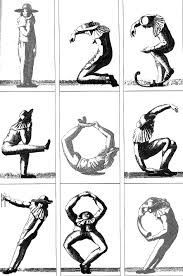
\includegraphics[width=10cm,height=13cm]{illustration1.jpg}
	\caption[Illustration 1]{Nombres entiers}
	\label{ill1}
\end{center}
\end{figure}
\end{center}

\newpage
\textbf{L}e codage d'entier naturel\index{Entier naturel} est l'un des rares cas o\`u il existe un code canonique\index{Code cannonique}~\cite{Cours_intro_info}.\newline
Le principe est le suivant : Convertir la valeur enti\`ere de base 10, en base 2.\newline
Le syst\`eme de num\'eration \`a base 2 ou encore syst\`eme binaire\index{Syst\`eme binaire} est un moyen de repr\'esenter les nombres avec 2 symboles : 0 et 1.\newline   Selon sa place, le symbole indique la pr\'esence d'une puissance de 2 (1) ou non (0). 
\newline Exemple : 1101 en binaire vaut 13  en base 10 :
\newline
\begin{figure}[H]
\begin{center}
	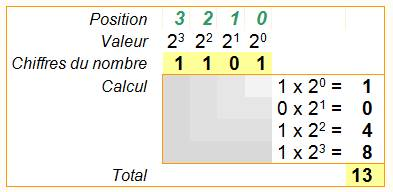
\includegraphics[height=4cm]{image1.jpg}
	\caption[Exemple 1]{Exemple de tableau d'encodage et de d\'ecodage binaire/d\'ecimal}
	\label{fig:ex1}
\end{center}
\end{figure}
La figure \ref{fig:ex1} est un exemple de conversion de base 2 en base 10~\cite{Entier_naturel}
\newline Cependant, le stockage de l'entier naturel varie en fonction de la valeur. En informatique, on stocke 1 symbole dans 1 bit\index{Bit}. 1 octet contient 8 bits. De ce fait, plus l'entier est grand, plus la conversion en base 2 comportera de symboles et donc utiliserons plus de m\'emoire.\newline 
\newline Pour information :
\begin{itemize}
\item 1 octet (byte)\index{byte} code les entier de 0 \`a 255
\item 2 octets (word ou short)\index{word}\index{short} code les entiers de 0 \`a 65 535
\item 4 octets (int)\index{int} code les entiers de 0 \`a 4 294 967 295
\item 8 octets (long)\index{long} code les entiers de 0 \`a 18 446 744 073 709 551 615 (18 milliards de milliards)
\end{itemize}

%%%%%%%%%%%%%%%%%%%%%%%%%%%%%%%%%%%%%%%%%%%%%%%%%%%%%%%%%%%%%%%

\newpage
\section{Codage de nombres relatifs}
\begin{center}
~\newline
\begin{figure}[h]
\begin{center}
	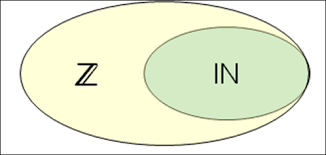
\includegraphics[width=11cm,height=11cm]{illustration2.png}
	\caption[Illustration 2]{Nombres relatifs}
	\label{ill2}
\end{center}
\end{figure}
\end{center}


\newpage
\textbf{L}e principe d'encodage et de d\'ecodage des entiers relatifs\index{Entier relatif} est le m\^eme que celui des entiers naturel sauf que le premier bit est utilis\'e pour repr\'esenter le signe du nombre~\cite{Entier_relatif}: 
\begin{itemize}
\item 0 pour le signe plus
\item 1 pour le signe moins
\end{itemize} 
~\newline
Si l'on prend l'exemple d'un octet, on a alors un bit de signe et sept bits pour coder la valeur absolue du nombre. Dans ce cas, un m\^eme octet peut repr\'esenter un nombre entre -127 et +127.\newline
\newline Exemple de codage sur un octet :
\begin{center}
\begin{tabular}{c|c}
Base 10 & Binaire\\
\hline
+82 &   0 1010010\\
-82 &  1  1010010\\
\end{tabular}
\end{center}
~\newline
Les deux repr\'esentations de 0 sur 1 octet avec la m\'ethode du bit de signe  sont : \og 0  0000000 \fg{} et \og 1  0000000 \fg{} (+0 et -0). Ce codage pr\'esente deux d\'efauts :
\begin{enumerate}
\item L'addition est complexe (il faut traiter quatre cas)
\item Le z\'ero a deux repr\'esentations 
\end{enumerate}
Pour ces raisons la m\'ethode du bit de signe seul n'est (presque) plus utilis\'ee.\newline
\newline Pour information :
\begin{itemize}
\item 1 octet (byte) code de -128 \`a 127
\item 2 octets (short) code de -32 768 \`a 32 767 
\item 4 octets (int) code de  $-2^{31}$ \`a $2^{31}$ 
\item 8 octets (long) code de $-2^{63}$ \`a $2^{63}$ 
\end{itemize}

%%%%%%%%%%%%%%%%%%%%%%%%%%%%%%%%%%%%%%%%%%%%%%%%%%%%%%%%%%%%%%%

\newpage
\section{Codage de r\'eels}
\begin{center}
~\newline
\begin{figure}[h]
\begin{center}
	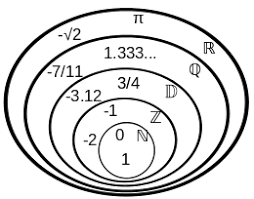
\includegraphics[width=11cm,height=13cm]{illustration3.png}
	\caption[Illustration 3]{Nombres r\'eels}
	\label{ill3}
\end{center}
\end{figure}
\end{center}

%%%%%%%%%%%%%%%%%%%%%%%%%%%

\subsection{Codage en virgule fixe}
\paragraph{Principe}
\textbf{L}e principe du codage \`a virgule fixe\index{Virgule fixe} est simple : Chaque r\'eel est encod\'e par 2 entiers :  la partie enti\`ere et la partie fractionnaire.
Pour le codage de la partie fractionnaire, les puissances de 2 seront n\'egatives et on ira de la plus grande \`a la plus faible puissance. Pour y voir plus claire, rien de mieux qu'un exemple.\newline
~\newline 10,625 (en base 10) : 
\newline = 8 + 2 + 0.5 + 0.125 
\newline = $1*2^{3} + 0*2^{2} + 1*2^{1} + 0*2^{0} + 1*2^{-1} + 0*2^{-2} + 1*2^{-3}$
\newline  = 1010.101 (en binaire) 
~\newline
\newline On peut d\'emonter rigoureusement que tout nombre r\'eel positif inf\'erieur \`a 1
pourrait \^etre \'ecrit de cette mani\`ere.~\cite{Codage_virgule_fixe}
Resterait \`a d\'ecrire le signe, ce qui peut \^etre fait par un bit particulier (bit de signe)
ou par une convention.
\paragraph{Point technique} Pour coder la partie fractionnaire d'un r\'eel de base 10 en binaire, on peut multiplier le nombre par deux. Si le produit obtenu est inferieur \`a 1, on ajoute un 0 \`a la conversion, sinon on ajoute un 1. Ensuite, on prend la partie d\'ecimal du produit et on recommence, ainsi de suite jusqu'\`a obtenir un produit \'egale \`a 1. 
\newline Prenons pour exemple le codage de 0,625:
\begin{enumerate}
\item $0.625*2 = 1.25 > 1$ On pose : $0,625_{10} = 0,1..._{2}$
\item $0,25*2 =  0,5 < 1$ On pose : $0,625_{10} = 0,10..._{2}$
\item $0,5*2  =  1 =  1$ On pose : $0,625_{10} = 0,101_{2}$
\end{enumerate}

%%%%%%%%%%%%%%%%%%%%%%%%%%%%%

~\newpage
\subsection{Codage en virgule flottante}\index{Virgule flottante}
\paragraph{Base}\textbf{C}e codage est bas\'e sur la notation scientifique des r\'eels\index{Notation scientifique}.
Notation scientifique en base 10\index{Base 10,notation scientifique } :
Exemple : $123.456 = 1.23456 * 10^2$ 
\newline Plus g\'en\'eralement : N = $(-1)^S * M * 10^E$,  avec S $ \in $ \{0,1\} appel\'e "signe",  M $\in $ [1,10[ appel\'e "mantisse" et E $\in $ Z appel\'e "exposant".
\newline Probl\`eme : Comment encoder le z\'ero ? 
\newline Notation scientifique en base 2\index{Base 2, notation scientifique } :
Exemple : $1010.101 = 1.010101 * 2^3$ 
\newline Standard actuel : Norme IEEE 754 (2008) 
\newline N = $(-1)^S * M * 2^{E - B}$, avec S $\in $ \{0,1\},  M $\in $ [1,2[,  E et B $\in $ N
\newline Rem : B, appel\'e "biais", sert \`a obtenir des exposants n\'egatifs (sa valeur est fix\'ee par la norme)
\newline La norme IEEE 754 de 1985, revisit\'ee en 2008, d\'efinit 3 format de base~\cite{Norme_IEEE754} :
\begin{enumerate}
\item Le format simple \`a 32 bits
\item Le format double \`a 64 bits
\item Le format quadruple \`a 128 bits
\end{enumerate}
~\newline
On a donc :\newline \newline
\begin{tabular}{|c|ccc|c|}
\hline
format & Signe & Mantisse & Exposant & $Exposant_{max}$ \\
\hline
32 bits & 1 bit & 23 bits & 8 bits & 127\\
\hline
64 bits & 1 bit & 52 bits & 11 bits & 1023\\
\hline
128 bits & 1 bit & 112 bits & 15 bits & 16383\\
\hline 
\end{tabular}

\newpage
\paragraph{Principe}\textbf{U}ne fois apr\`es converit en notation scientifique de base 2 le r\'eel, on code le signe (0 ou 1). On code la mentisse, en enlevant le premier bit (qui est forc\'ement 1) par convention. Pour coder l'exposant selon la norme, il suffit de coder l'addition de l'exposant et de l'exposant maximum du format utiliser~\cite{Norme_IEEE754(2)}~\cite{Codage_virgule_fixe} .
\newline Pour finir la conversion, les bits cod\'es se rangent dans l'ordre suivant : 1)bit de signe ; 2)bits d'exposant ;
\newline 3) bits de mantisse.\newline
\newline Exemple : Coder -18,75 en 32 bits.~\cite{Codage_ieee754} \newline
\newline 18.75 $_{10}$ = 10010.110 $_{2}$ = $1.0010110*2^{4}$~$_{2}$
\begin{enumerate}
\item Signe = N\'egatif = 1 $_{2}$
\item Exposant = 4 $_{10}$ ; 4 + 127 = 10000011 $_{2}$
\item Mantisse = 0010110 $_{2}$ =  001~0110~0000~0000~0000~0000$_{2}$ (au format 32 bits)
\end{enumerate}
~\newline D'o\`u -18,75 $_{10}$ = 1~10000011~00101100000000000000000$_{2}$ selon la norme IEEE 754 au format 32 bits.


%%%%%%%%%%%%%%%%%%%%%%%%%%%%%%%%%%%%%%%%%%%%%%%%%%%%%%%%%%%%%%%

\newpage
\bibliographystyle{plain}
\bibliography{bibliography}

%%%%%%%%%%%%%%%%%%%%%%%%%%%%%%%%%%%%%%%%%%%%%%%%%%%%%%%%%%%%%%%

\newpage
\printindex

%%%%%%%%%%%%%%%%%%%%%%%%%%%%%%%%%%%%%%%%%%%%%%%%%%%%%%%%%%%%%%%

\newpage
\listoffigures

%%%%%%%%%%%%%%%%%%%%%%%%%%%%%%%%%%%%%%%%%%%%%%%%%%%%%%%%%%%%%%%

\end{document} 